%! TEX program = xelatex
\documentclass[12pt, twoside]{article}
\usepackage[a4paper, top=2.5cm, bottom=2.5cm, left=4cm, right=2.5cm]{geometry}
\usepackage{amsmath}
\usepackage{natbib}
\renewcommand{\bibname}{\centering References}
\usepackage{graphicx}
\usepackage{xeCJK}  
\usepackage{multicol}
\usepackage{setspace}
\usepackage{indentfirst}
\setlength{\parindent}{0.5in}
\usepackage{titlesec}
\titleformat*{\section}{\normalsize\bfseries\centering}
\titleformat*{\subsection}{\normalsize\bfseries}
\usepackage{booktabs, caption}
\usepackage{tikz}
\DeclareCaptionLabelSeparator*{spaced}{\\[2ex]}
\captionsetup[table]{textfont=it,format=plain,justification=justified, 
	singlelinecheck=false,labelsep=spaced,skip=0pt}
\captionsetup[figure]{labelsep=period,labelfont=it,justification=justified, 
	singlelinecheck=false,font=doublespacing}
\setCJKmainfont{PMingLiU}
\setmainfont{Times New Roman}

% Begin the document

\begin{document}

    \doublespacing
    \begin{titlepage}
    \begin{figure}
        \centering
        \includegraphics[width=8cm]{Title/UM_logo.png}
%        \caption*{}
%        \label{fig:um}

    \end{figure}
    \smallskip
    \begin{center}
        \Large
        教育學院 \\
        Faculty of Education \\
    \end{center}
    \smallskip
    \begin{center}
    	% Your major here. 
        哲學碩士學位課程(專業名稱) \\
        Master of Philosophy (Name of Major)
    \end{center}
    \smallskip
    \begin{center}
    	
        \large
        論文題目 \\ 
        Thesis Title \\ 
        
         
    \end{center}
    \vfill
    \begin{flushleft}
        \begin{multicols}{2}
        	% Your name here
            學生姓名: \\
            學生編號: \\
            指導教授:\\
            \columnbreak
            Student Name:  \\
            Student No:  \\
            Supervisor Name:  \\
        \end{multicols}
    \end{flushleft}
    \smallskip
    \begin{center}
    	% Your oral defence date here
        答辯日期 (年/月) \\
        
    \end{center}
\end{titlepage}
\newpage
    \newpage

    % Acknowledgements
    \pagenumbering{roman}
    \section*{\centering Acknowledgments}
\addcontentsline{toc}{section}{Acknowledgments}
\begin{spacing}{2}
    Your acknowledgment goes here.  
    
    \smallskip
    
    \rightline{Your name here}
    \rightline{Date}
    
    \newpage
    
    \section*{\centering 致謝(中文版)}
    \smallskip
    
    \par
    你也許會想要寫一點中文的東西.
    
    以及, 若你想感(追)謝(殺)一下這個模板的作者森珞璃子也不是不行啦. 雖然我覺得應該沒什麼人會用 \LaTeX 折磨自己就是了. 
    
    當然也讓我稍微感謝一下桜坂璃子. 
    
    \par
    如果不需要的話整個section刪掉就好啦.
    
    \rightline{君の名は}
    \rightline{日期}
    
\end{spacing}
    \section*{\centering Abstract}
\addcontentsline{toc}{section}{Abstract}
\begin{spacing}{2}
	\noindent
    Your abstract with startling originality. 
\end{spacing}

\smallskip

\begin{spacing}{2}
    \textit{Keywords: } your, cool, keywords
\end{spacing}
    \section*{\centering Declaration}
\addcontentsline{toc}{section}{Declaration}
\begin{spacing}{2}
    \par
    I declare that the thesis here submitted is original except for the source materials explicitly acknowledged and that this thesis as a whole, or any part of this thesis has not been previously submitted for the same degree or for a different degree. 
    \par
    I also acknowledge that I have read and understood the Rules on Handling Student Academic Dishonesty and the Regulations of the Student Discipline of the University of Macau.
\end{spacing}

    % ToC
    \renewcommand*\contentsname{\centering Table of Contents}
    \tableofcontents
    \newpage
    
    \renewcommand{\listtablename}{\centering List of Tables}
    \listoftables
    \addcontentsline{toc}{section}{List of Tables}
    \newpage
    
    \renewcommand{\listfigurename}{\centering List of Figures}
    \listoffigures
    \addcontentsline{toc}{section}{List of Figures}
    \newpage

    % include your chapters here. 
    \pagenumbering{arabic}
    \section{Introduction}
\begin{spacing}{2}
    \par
    Driven by escalating competition in traditional educational settings, the prevalence of supplementary tutoring beyond the standard school schedule has surged, becoming a prevalent tactic for students striving to secure an advantageous position in scholastic endeavors. It is extensively acknowledged that students hailing from lower socioeconomic status (SES) families tend to underperform academically compared to their higher-SES counterparts. \citep{zhou2015family}.  
    
    \par
    Show your research objectives by bulleted or numbered list. 
    
    \begin{enumerate}
        \item This is my first point. 
        \item This is my second point. 
        \item And my third research objective. 
    \end{enumerate}
    
    \par
    
    \subsection{Table}    
    \par
    Talk is cheap, now show me the data! 
    
    \begin{table}[h]
    	\caption{A Table Demo}
    	\begin{tabular}{l c c c c}
    		\toprule
    		Column 0 & Column 1 & Column 2 &  Column 3 & Column 4 \\
    		\midrule
    		Row 0 		& 1 & 12.05 & 4.60\% & 71.68 \\
    		Row 1 		& 117 & 81.88 & 96.58\% & 1.71 \\
    		Row 2 		& 15 & 84.93 & 100\% & 0.00 \\
    		Row 3 		& 343 & 61.49 & 61.81\% & 20.12 \\
    		Row 4 		& 242 & 73.92 & 94.21\% & 0.83\ \\
    		Row 5 		& 99 & 70.83 & 87.88\% & 0.00  \\
    		Row 6 		& 117 & 64.10 & 74.36\% & 0.00  \\
    		Row 7 		& 344 & 80.44 & 94.48\% & 0.29 \\
    		\bottomrule
    	\end{tabular}
    \end{table}
    
    \subsection{Figure, and my own thoughts}
    %REMOVE THESE IF YOU WANT TO GET YOUR DEGREE
    \par
    As you find this repository, you must would like to try this beautiful document preparation language. But, listen to me: 
    \begin{center}
    	\large
    	DON'T
    \end{center}
    
    My engagement with \LaTeX \ somewhat mirrors an encounter in a covert, dimly-lit underground chamber. Enveloped in my vintage Lolita attire - appearing every inch the doll - I dangle aloofly from the ceiling. My eyes glaze with a touch of helpless desperation as I am punished repeatedly with errors each time I dare to compile my document.
    
    Yet, in the throes of this torturous process, I find myself crying out for more – more – MORE! Let this not be a path you choose to tread. \textbf{Employ a WYSIWYG editor if feasible.} However, if the siren call of this forbidden yet exciting relationship proves irresistible and you yearn to surrender to this seductive creature, opt for using \verb|R Markdown| instead. By all means, spare your thesis from the clutches of \LaTeX.
    
    %REMOVE THESE IF YOU WANT TO GET YOUR DEGREE
    
    \begin{figure}
    	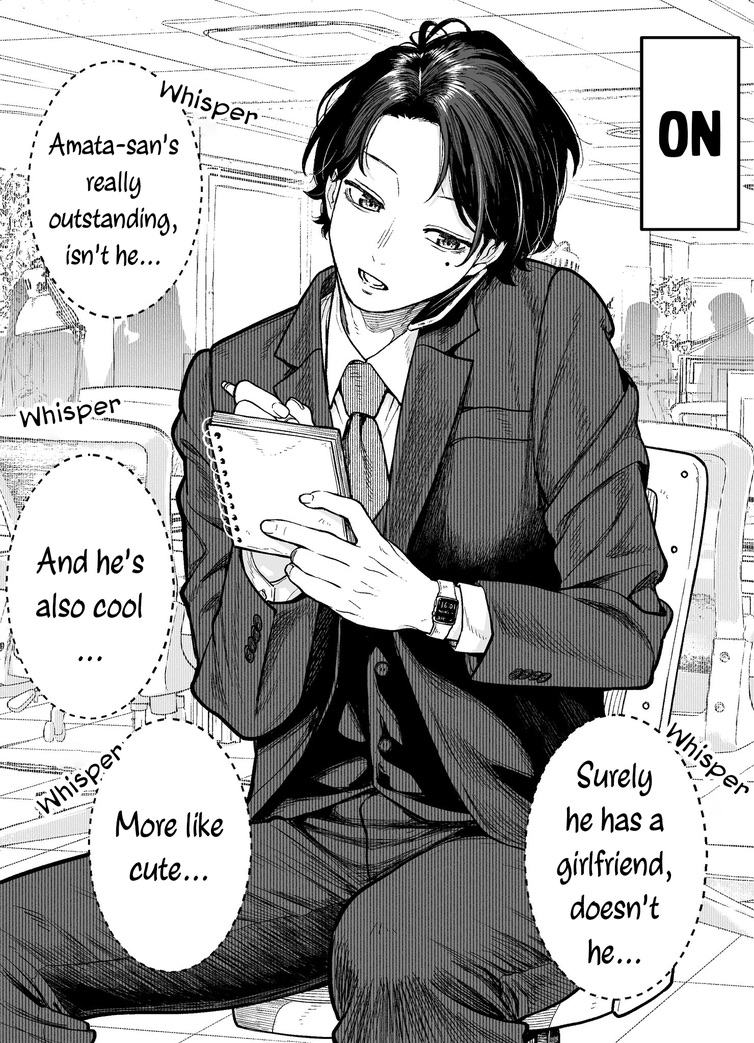
\includegraphics[width=0.4\textwidth]{ch1/on-mode.jpg}
    	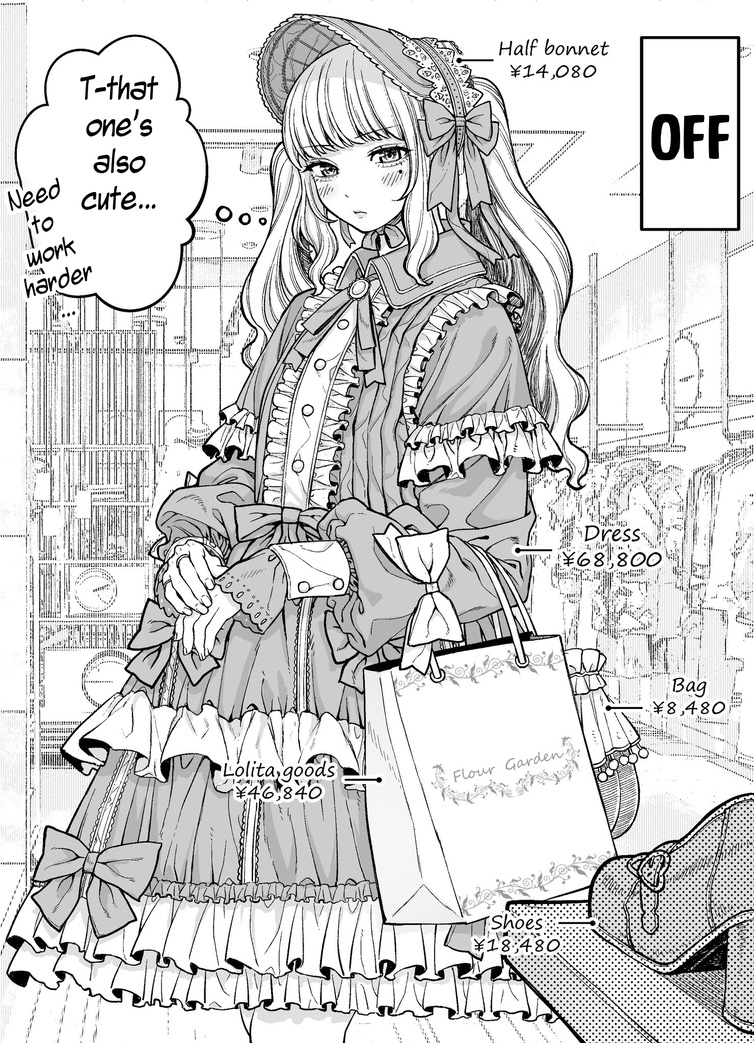
\includegraphics[width=0.4\textwidth]{ch1/off-mode.jpg}
    	\caption{Amata-san's ON and OFF mode. }
    \end{figure}

    \subsection{Another subsection}
    
    \par
    But text only. 
    
\end{spacing}
    \newpage
    
    % include{Ch2/ch2.tex}
    % \newpage
    
    \bibliography{references}
    \addcontentsline{toc}{section}{References}
    \bibliographystyle{apalike}

\end{document}